% !TEX encoding = UTF-8 Unicode
\documentclass[a4paper]{article}

\usepackage[utf8]{inputenc}
\usepackage{erk}
\usepackage{cite}
\usepackage{tikz}
\usepackage{times}
\usepackage{graphicx}
%\usepackage{graphicx}
\usepackage[outdir=./]{epstopdf}
%\usepackage{caption}
\usepackage{subcaption}
\usepackage[top=22.5mm, bottom=22.5mm, left=22.5mm, right=22.5mm]{geometry}
\usetikzlibrary{shapes, fit, arrows, calc, positioning}

\tikzstyle{block} = [draw, rectangle, minimum width = 0.75cm, minimum height = 0.75cm]
\tikzstyle{sum} = [draw, circle, minimum size=.5cm, node distance=1.75cm]
\tikzstyle{input} = [coordinate]
\tikzstyle{output} = [coordinate]
\tikzstyle{support} = [coordinate]
% USER DEFINED MACROS
\newcommand{\matlab}{MATLAB\textsuperscript{\textregistered}}
\newcommand{\simulink}{SIMULINK\textsuperscript{\textregistered}}
\newcommand{\matsim}{MATLAB\textsuperscript{\textregistered} SIMULINK\textsuperscript{\textregistered}}
\newcommand{\thom}{$\textbf{T}^i_{i+1}$}
\newcommand{\Lagrt}{\mathcal{T}}
\newcommand{\Lagrl}{\mathcal{L}}
\newcommand{\Lagru}{\mathcal{U}}
\usepackage[slovene,english]{babel}

\hyphenation{spre-mem-be}


% local definitions
\def\footnotemark{}%  to avoid footnote on cover page

\begin{document}
%make title
\title{UDP-ARCNET strežnik za krmiljenje robota PA-10}

\author{Timotej Gašpar$^{1}$, Leon Žlajpah$^{2}$} % use ^1, ^2 for author(s) from different institutions

\affiliation{$^{1}$Fakulteta za elektrotehniko\\ 
$^{2}$Institut »Jožef Stefan«}

\email{E-pošta: timotej.gaspar@gmail.com}

\maketitle

%\thispagestyle{empty}

\begin{abstract}{UDP-ARCNET server for control of PA-10 robot}

Servo motor controllers of industrial robots usually allow the users very limited control. Manufacturers usually do not provide detailed information on the low level motor control. On the other hand, Mitsubishi Portable Intelligent Arm PA-10 comes with a good documentation on the servo driver, and allows the user to know all the parameters of servo motor regulation. The servo also allows the user to control each motor separately in velocity or torque mode, opening various options in terms of control. The servo controller has an ARCNET module for communication in the ARCNET network, through witch the user can access and set the control parameters and motor control.

When designing end point robot control, the faster the control frequency is, the better performance one can achieve. 

We implemented a UDP-ARCNET server as a man-in-the-middle for servo controller communication with the wish to achieve high control frequencies. The server allows control frequencies up to 500 Hz. It was built on Linux operating system in the low level programming language C.

The server allows the users to control the robot via custom programs that allow UDP communication. For evaluation purposes of the server, admittance control is implemented and tested.

\end{abstract}


\selectlanguage{slovene}

\section{Uvod}

Raziskovalne institucije, ki raziskujejo algoritme vodenja robotov, pogosto uporabljajo industrijske robote. Med razvijanjem algoritmov je pomembno dobro poznavanje dinamičnih parametrov robota ter delovanje krmilnika, vendar podjetja, ki proizvajajo industrijske robote, v večini ne nudijo uporabnikom vseh podatkov.

Podjetje Mitsubishi Heavy Industries je leta 1992 izdelalo prvega katalogiranega industrijskega redundantnega robota, Portable General-purpose Intelligent Arm PA-10 \cite{mhi_pa10}. Gre za serijskega robota s sedmimi stopnjami prostosti. Masa robotske roke PA-10 je 36 kg in ima nosilnost 10 kg. Servo motorji v sklepih se napajajo preko izmenične napetosti. Prenosi v sklepih so realizirani z harmoničnimi gonili. Baza robota da se lahko pritrdi v katerokoli lego. To pomeni, da se ga lahko fiksira bodisi na tla, na steno ali na strop. Robota PA-10 odlikuje relativno lahka konstrukcija, enostavno rokovanje ter odprtost njegovega krmilnika. Prav ti razlogi so povod, da mnogo instituciji uporablja robota kot eksperimentalni sistem za razvijanje algoritmov vodenja robotov (\cite{voung_pa10}, \cite{aalst_pa10}, \cite{rodrigo_pa10},\cite{petric_nevronska}).

Nekatere naloge zahtevajo interakcijo robota z okoljem s določeno silo. S poznavanjem vseh dinamičnih parametrov je v teoriji mogoče izračunati sile, ki delujejo na vrh robota. V praksi se izkaže, da te parametre ni vedno mogoče dovolj natančno definirati. Iz teh razlogov se vgradi senzor sil in navorov med vrhom robota ter prijemalom (\cite{almassri_pressure_sensor}, \cite{mihelj_vodenje}, \cite{eppinger_force_dynamics}). Tako se lahko vodi robota preko inverzne dinamike z upoštevanjem izmerjenih sil. Tako vodenje imenujemo admitančno vodenje \cite{mihelj_hapt}.
%\section{Robotski mehanizem PA-10}

	
\section{UDP-ARCNET strežnik}

Proizvajalec Mitsubishi Heavy Industries je za upravljanje in programiranje robota pripravil posebno programsko opremo. Iz dokumentacije je razvidno, kaj vse je njihova programska oprema omogočala. Težava pa je, da omenjena programska oprema ni več dostopna. Proizvajalec je s prodajo robotov PA-10 prenehal v letu 2009, s podporo pa v marcu 2014 (vir: osebno dopisovanje s proizvajalcem). 

\subsection{Krmilnik servo motorjev robota} \label{sec:servo-drive}

V ohišju servo krmilnika so vgrajeni štirje krmilniki servo motorjev. Vsak servo krmilnik krmili dva servo motorja, razen enega. Krmilniki omogočajo vodenje motorjev na dva načina: navorno in hitrostno. Navorno vodenje je realizirano z analognim P regulatorjem toka, hitrostna regulacija pa je realizirana z digitalnim PI regulatorjem s frekvenco približno 1500 Hz.

Krmilnik vsebuje dva pomnilnika. Delovni pomnilnik (RAM) in nastavitveni pomnilnik (EEPROM). V EEPROM tabeli so zapisani parametri za nastavitve in vodenje servo krmilnikov. Ob zagonu krmilnika se parametri naložijo iz EEPROM tabele v RAM. Med temi parametri so tudi ojačanje proporcionalnega ter integracijskega dela regulatorja, omejitve posameznih stopenj, razmerje prenosa zobnikov, itd.

\subsection{ARCNET vmesnik}\label{sec:arc_drive}

Referenčne navore in hitrosti se na krmilniku nastavlja preko zunanjega vmesnika, ki je povezan na enako ARCNET omrežje kot servo krmilnik. ARCNET je omrežje, ki vključuje podatkovni in fizični nivo po OSI modelu, komunikacija po omrežju pa je serijska in paketno zastavljena. Njegova prednost pred Ethernet omrežjem je velika stopnja determinističnosti \cite{arc_tutorial}. Krmilnik ima dva priključka za optični 
vodili, vhod (Rx) ter izhod (Tx). Zgornja meja hitrosti komunikacije z krmilnikom robota PA-10 je 5 Mb/s \cite{pa10-manual}.

\subsection{Senzor sile in navorov - JR3}	

Na vrh robota smo pritrdili senzor sil in navorov JR3. Senzor omogoča merjenje sil in navorov v $x$, $y$ in $z$ oseh. Uporovni lističi porazdeljeni po notranjosti senzorja se deformirajo pod vplivom sile. Upornost na uporovnih lističih spremeni proporcionalno s silo, ki deluje na senzor. Sprememba upornosti se izmeri posredno preko spreme\-mbe napetosti na AD-pretvorniku, ki je vgrajen v sam senzor. 

Senzor se priključi preko 6 ali 8 žilnega vodila na računalniško kartico. Senzor serijsko pošilja podatke o izmerjenih silah na kartico. Kartica vsebuje vezje za digitalno obdelavo signalov. V dokumentaciji kartice \cite{jr3_doc_inst} so opisani trije nizkoprepustni filtri z različnimi mejnimi frekvencami. Uporabili smo filter z mejno frekvenco 500 Hz.

Na računalniku je bila nameščena kartica na vodilu ISA. Ker je standard starejši, je podjetje prenehalo s podporo tega standarda. Kot posledica tega smo dela razvili svojo programsko opremo za komunikacijo z notranjimi registri kartice.

\subsection{Strežnik} \label{sec:streznik}

\begin{figure}[!t]
	\centering
	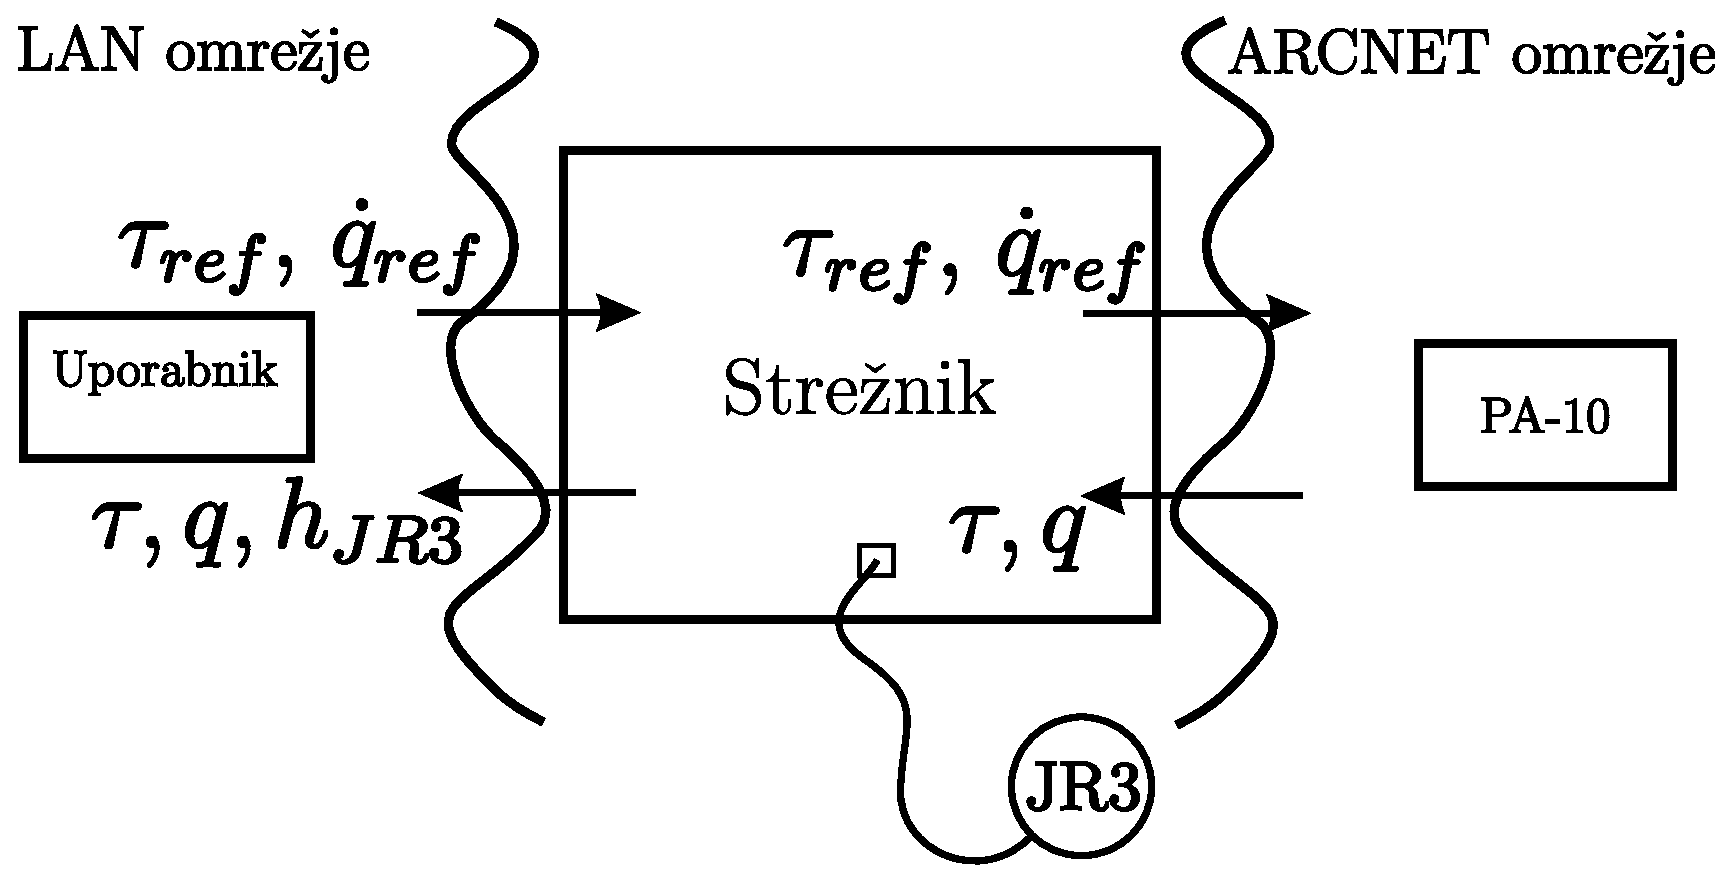
\includegraphics[width=0.4\textwidth]{./slike/udp-arcnet-server.eps}
	\caption{Strežnik kot posrednik med dvema omrežjema}
	\label{fig:server}
\end{figure}

Pred začetkom izdelave lastnega programskega orodja se je definiralo dve zahtevi. Prva je bila, da program deluje kar se le da hitro in kar se le da v realnem času. To izhaja iz vidika stabilnosti vodenja. Mihelj v \cite{mihelj_hapt} namreč navaja, da vzorčni čas močno vpliva na stabilnost vodenja robota v kontaktu z okolico. Večja kot je vzorčna frekvenca večja je lahko togost okolice s katero je robot v kontaktu.

Druga zahteva pa je bila enostavna uporaba. Želeli smo, da uporaba programske opreme, ki jo naredimo, zahteva čim manj predznanja o komunikacijskih protokolih po ARCNET mreži. Hkrati pa mora program omogoča\-ti neko mero svobode pri realizaciji visoko nivojskega vodenja.

Dodatno se je kasneje pojavila še želja, da bi programska oprema omogočala tudi posredovanje meritev izvedenih na senzorju sile JR3. Tako bi nastal program, ki bi komuniciral tako s servo kontrolerjem kot z ISA kartico za senzor sile JR3.

Naštete zahteve so privedle do izbire primernega operacijskega sistema in programskega jezika. Razvili smo strežnik v programskem jeziku C na operacijskem sistemu Linux. Strežnik deluje kot posrednik med dvema različnima omrežjema, ARCNET in Ethernet (slika \ref{fig:server}). Stre\-žnik je nastavljen za delovanje s časovnim ciklom $2$ ms. Standardna deviacija od nastavljenega programskega cikla na strežniku je  $\pm 0.00086 $ ms. Časovni potek časovnega cikla med delovanjem programa prikazuje slika \ref{fig:jittergraph}.

\begin{figure}[!h]
	\centering
	\includegraphics[width=0.5\textwidth]{./slike/figure_jitter}
	\caption{Odstopanje programskega cikla med delovanjem strežnika}
	\label{fig:jittergraph}
	
\end{figure}

\section{Admitančno vodenje}

Vodenje robota preko vhodnih hitrostih v sklepih uporablja PI regulator v krmilniku, ki poskrbi, da se vsak sklep vrti s hitrostjo čimbolj podobno referenčni. Iz tega vidika je prednost ta, da ne glede na konfiguracijo ter obremenitev robota, bo regulator vedno poskrbel čim boljše sledenje referenci. Vplivi gravitacije se kompenzirajo z integrirnim členom v regulatorju. 


\subsection{Vodenje v notranjih koordinatah} \label{sec:admit_inner}

Krmilnik servo motorjev nam v vsakem danem trenutku vrača trenuten kot v sklepu. Ker ima PI regulator visoka ojačanja ter visoko frekvenco, bomo za namene poenostavitve aproksimirali motor kot integrator $\frac{1}{s}$. Naj bo referenčni kot v sklepih označen z $\textbf{q}_{\mathrm{ref}}$ in naj bo dejanski kot označen z $\textbf{q}$. Razlika med njima je napaka v kotu 

\begin{equation}
\tilde{\textbf{q}} = \textbf{q}_{\mathrm{ref}} - \textbf{q}.
\end{equation}
S preprostim P regulatorjem lahko kote v sklepu robota vodimo s povratno zanko. Ojačanje regulatorja bo označe\-no s $\textbf{K}_p$, ki je diagonalna matrika, saj ima vsak sklep svoje ojačanje neodvisno od ostalih. S povečevanjem ojačanja regulatorja \textbf{K} vplivamo na dinamiko odziva.

\begin{equation} \label{eq:p_reg_q}
\textbf{u} = \textbf{K}_p  \tilde{\textbf{q}}.
\end{equation}


Za boljšo stabilnosti vnesemo še signal dušenja $\textbf{K}_d \dot{\mathbf{q}}$. Matrika $\textbf{K}_d$ je tako kot $\textbf{K}_p$ diagonalna. Regulirni signal sedaj zapišemo z

\begin{equation} \label{eq:pd_reg_q}
\textbf{u} = \textbf{K}_p \tilde{\mathbf{q}} - \textbf{K}_d \dot{\mathbf{q}}.
\end{equation}

\subsection{Vodenje v zunanjih koordinatah} \label{sec:admit_out}

Naj bo $\textbf{x}_{\mathrm{ref}}$ vektor referenčne lege vrha robota in naj bo $\textbf{x}$ trenutna lega vrha robota. Napaka je tako

\begin{equation} \label{eq:xerr}
\tilde{\textbf{x}} = \textbf{x}_{\mathrm{ref}}  - \textbf{x}
\end{equation}

Enačba direktne kinematike nam govori o odnosu med hitrostjo vrha robota ter hitrostjo v sklepih robota

\begin{equation} \label{eq:qtox}
\dot{\textbf{x}} = \textbf{J}(\textbf{q})  \dot{\textbf{q}}.
\end{equation}

To enačbo je mogoče razumeti tudi kot zvezo med spremembo položaja vrha ter sklepov robota \cite{mihelj_vodenje}. Zato je mogoče to enačbo uporabiti za zapis relacije med napako vrha ter potrebnim odmikov v sklepih preko enačbe za inverzno kinematiko

\begin{equation} \label{eq:qerr}
\tilde{\textbf{q}} = \textbf{J}^{\#}(\textbf{q})  \tilde{\textbf{x}}.
\end{equation}
$\mathbf{J}^{\#} =  \mathbf{J}^{T} (\mathbf{J} \mathbf{J}^T)^{-1}$ je generaliziran pseudoinverz Jacobijeve matrike.

Z vstavitvijo enačbe (\ref{eq:qtox}) v (\ref{eq:p_reg_q}) dobimo P regulator lege vrha robota Sedaj je mogoče regulirni signal, ki krmili hitrost v sklepih robota tako, da bo vrh sledil referenčni legi

\begin{equation} \label{eq:outcontrol}
\textbf{u} = \textbf{K}_p  \textbf{J}^{\#}(\textbf{q})  (\textbf{x}_{ref} - \textbf{x}).
\end{equation}

V \cite{mihelj_vodenje} je navedeno, da se mehanski sistem, ki je voden na ta način obnaša kot mehanski sistem z \textit{n} - dimenzionalno vzmetjo v notranjih koordinatah. Togost omenjene vzmeti pa določa ojačanje $\textbf{K}_p$.


\subsection{Admitančno vodenje} \label{sec:vodenje-admitance}

Robotski mehanizem PA-10 je industrijski robot s segmenti iz pretežno litega železa. Segmenti imajo relativno veliko maso, sklepi pa relativno visoko trenje. Lahko predpostavimo, da ima manipulator veliko lastno impedanco. Pojem mehanske impedance izvira iz analogije električne impedance. Predstavlja pa razmerje med silo (\textit{F}) in hitrostjo (\textit{v}) 

\begin{equation}
Z(s) = \frac{F}{v} = ms + b + \frac{k}{s}
\end{equation}
oziroma razmerje med silo in pozicijo (\textit{x})

\begin{equation}
Z(s) = \frac{F}{x} = ms^2 + bs + k,
\end{equation}
kjer je \textit{m} masa, \textit{b} viskozno dušenje, \textit{k} togost \cite{mihelj_hapt}.



Za admitančno vodenje je potrebno še upoštevati podatek o silah in navorih, ki delujejo na vrhu robota. Izmerjene sile in navori bodo označene s $\textbf{h}_{\mathrm{JR3}}$, referenčne sile in navori pa z $\textbf{h}_{\mathrm{ref}}$. Napaka sile je tako definirana kot:
\begin{equation} \label{eq:herr}
\tilde{\textbf{h}} = \textbf{h}_{\mathrm{ref}} - \textbf{h}_{\mathrm{JR3}}.
\end{equation}

Sila kot rezultat delovanja robota na okolico je odvisna od hitrosti oz. pozicije vrha robota. Premikal se bo v smeri želene sile. Zato lahko napako sile dodamo v regulator lege, podan z enačbo (\ref{eq:outcontrol}). Definiramo referenčno pozicijo v odvisnosti od hitrosti

\begin{equation} \label{eq:xrefforce}
\textbf{x}_{\mathrm{ref}} = \textbf{K}_{hP}\tilde{\textbf{h}} + \textbf{K}_{hI} \int_{0}^{t}\tilde{\textbf{h}}d\xi.
\end{equation}

Dobili smo PI regulator sile interakcije. Čeprav je bilo pri definiciji mehanske impedance definirano, da je to razmerje med silo ter hitrostjo, se raje uporablja razmerje med silo ter pozicijo. Meritve sile so podvržene šumu, integrator pa deluje kot nizkopasovni filter. Z vpeljavo integratorja, dosežemo to, da se bo robot premikal v smeri želene sile s hitrostjo $\textbf{K}_{hI} \tilde{\textbf{h}}$.

Z vstavitvijo enačbe (\ref{eq:xrefforce}) v (\ref{eq:outcontrol}) je mogoče zapisati celotno regulacijsko enačbo za vodenje robota v zunanjih koordinatah z upoštevanjem delovanja zunanjih sil na vrh robota.

\begin{equation} \label{eq:admitcontrol}
\textbf{u} = \textbf{K}_p  \textbf{J}^{\#}(\textbf{K}_{hP}\tilde{\textbf{h}} + \textbf{K}_{hI} \int_{0}^{t}\tilde{\textbf{h}}d\xi - \textbf{x})
\end{equation}


\section{Rezultati}
%\begin{figure}
%	\centering
%	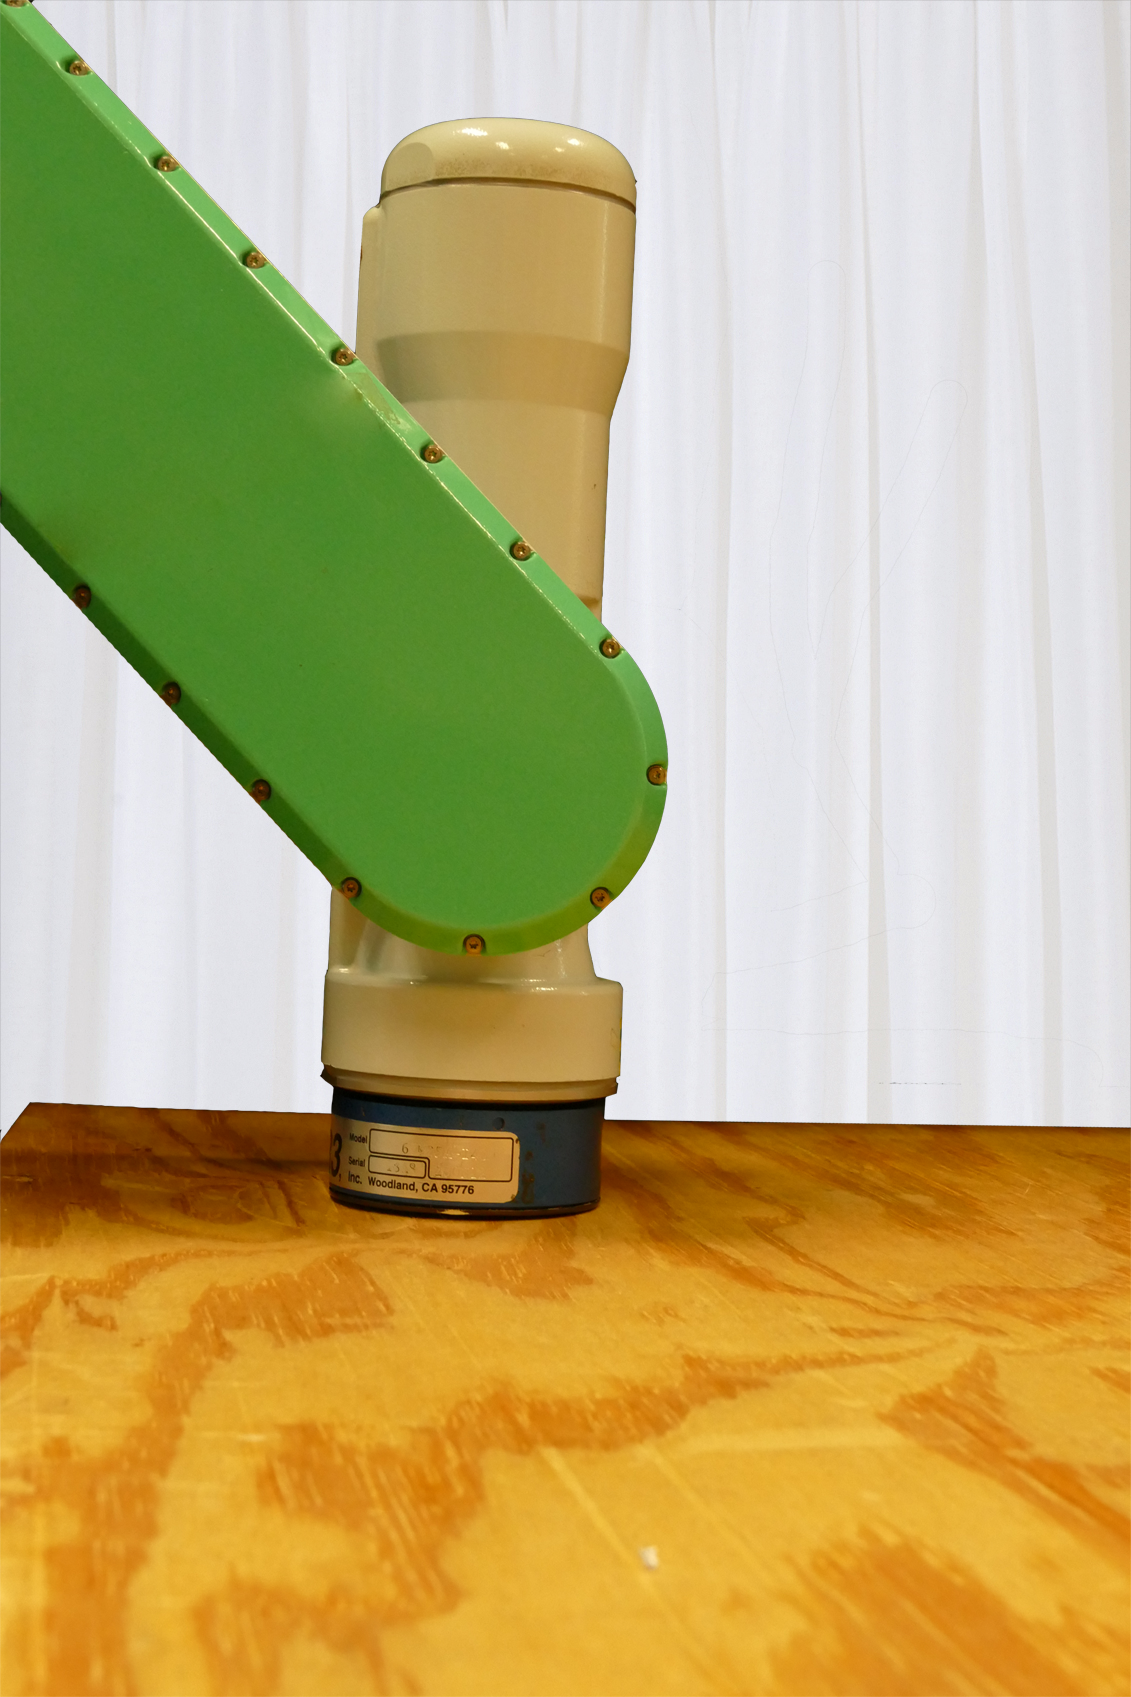
\includegraphics[trim=0.7cm 5cm 2cm 0cm,clip=true,width=0.4\textwidth]{./slike/pa10jr3.png}
%	\caption{Robot PA-10 in senzor sile JR3 v kontaktu s togo okolico.}
%\end{figure}

Zgrajen strežnik smo ovrednotili z vodenjem robota v kontaktu s togo okolico. Najprej je bil opravljen preizkus na vzbujanje s stopničasto funkcijo. Primerjali smo odzive robota na različno velikost stopnice pri različnih vzorčnih časih, 100 Hz ter 500 Hz.

\begin{figure}[!ht]
	
	   \begin{subfigure}[b]{0.4\textwidth}
	   	\includegraphics[width=\textwidth]{./slike/figure_0_hz_100dt.eps}

	   	\caption{Odziv na stopnico pri vzorčni frekvenci 100 Hz}
	   	\label{fig:0hzgraph100}
	   \end{subfigure}
	   ~ %add desired spacing between images, e. g. ~, \quad, \qquad, \hfill etc. 
	   %(or a blank line to force the subfigure onto a new line)
	   \begin{subfigure}[b]{0.4\textwidth}
	   	\includegraphics[width=\textwidth]{./slike/figure_0_hz_5.eps}
	   	\caption{Odziv na stopnico pri vzorčni frekvenci 500 Hz}
	   	\label{fig:0hzgraph500}
	   \end{subfigure}
	   	\caption{Odzivi dotik s togo okolico ob stopničastem referenčnem signalu}
	   	\label{fig:stepgraphs}
	
\end{figure}

Na sliki \ref{fig:stepgraphs} je razvidno, da je pri 100 Hz sistem pri enakih parametrih regulatorja, $K_{hP}$ in $K_{hI}$, ni več stabilen, saj odskakuje od podlage, kar je vidno v spremenljivi sili. Pri 500 Hz se lahko robot dotakne toge okolice in ohranja referenčno silo.

Nato smo ovrednotili vodenje strežnika s 500 Hz pri referenčnem signalu sinusne oblike. Rezultate pri različnih frekvencah sinusnega signala so prikazani na sliki \ref{fig:sineref}.

\begin{figure}[!ht]
	
\centering

	\begin{subfigure}[b]{0.4\textwidth}
		\includegraphics[width=\textwidth]{./slike/figure_5_hz.eps}
		\caption{Odziv na sinusni signal s frekvenco 0.5 Hz}
%		\label{fig:0hzgraph100}
	\end{subfigure}

	\begin{subfigure}[b]{0.4\textwidth}
		\includegraphics[width=\textwidth]{./slike/figure_10_hz.eps}
		\caption{Odziv na sinusni signal s frekvenco 1 Hz}
%		\label{fig:0hzgraph500}
	\end{subfigure}
	
	\begin{subfigure}[b]{0.4\textwidth}
		\includegraphics[width=\textwidth]{./slike/figure_20_hz.eps}
		\caption{Odziv na sinusni signal s frekvenco 2 Hz}
%		\label{fig:0hzgraph500}
	\end{subfigure}
	
	\caption{Odzivi ob kontaktu s togo okolico ob sinusnem referenčnem signalu}
	\label{fig:sineref}
\end{figure}

Iz grafov je videti, da robot dobro sledi referenci do frekvence sinusnega signala pod 1 Hz. Pri višjih frekvencah je napaka večja.

\section{Zaključek}

Vodenje robotov v kontaktu z togo okolico zahteva visoko vzorčno frekvenco. Admitančno vodenje omogoča vodenje sile vrha robota preko hitrosti v sklepih vendar je zato potrebno namestiti ustrezen senzor. Namenski strežnik, ki je bil zgrajen za vodenje robota PA-10 dosega zastavljene cilje. Hkrati pa omogoča prilagoditev na dodatne funkcije v kolikor bodo te v prihodnosti potrebne. Nadaljnje delo bo implementirati vodenje preko dinamičnega modela. 

\small

\bibliographystyle{ieeetr}
\bibliography{literatura}
%\begin{thebibliography}{1}
%
%\bibitem{ERK} ERK, http://www.ieee.si/erk/index.html 
%\bibitem{Zbornik} B. Zajc, A. Trost: Zbornik triindvajsete mednarodne Elektrotehniške in računalniške konference ERK 2014, 22. - 24. September 2014, Portorož, Slovenija
%
%
%
%\end{thebibliography}

	\end{document}
